\documentclass[a4paper,12pt]{article}

% ======================================================================
% PACKAGES ET CONFIGURATIONS
% ======================================================================
\usepackage[utf8]{inputenc}    % Encodage d'entrée, pour les caractères accentués
\usepackage[T1]{fontenc}       % Encodage de police
\usepackage{geometry}          % Gérer les marges
\usepackage{titlesec}          % Personnaliser les titres de sections
\usepackage[colorlinks=true,linkcolor=blue,urlcolor=blue]{hyperref} % Liens cliquables

\usepackage{listings}          % Pour insérer des listings de code
\usepackage{xcolor}            % Gestion des couleurs

% TikZ pour les diagrammes
\usepackage{tikz}
\usetikzlibrary{arrows.meta, shapes, positioning}

% Configuration des listings
% On définit l'apparence du code inséré
\lstset{
    basicstyle=\ttfamily\small,
    keywordstyle=\color{blue}\bfseries,
    commentstyle=\color{gray},
    stringstyle=\color{orange},
    showstringspaces=false,
    columns=fullflexible,
    frame=single,
    breaklines=true,
    numbers=left,
    numbersep=5pt,
    aboveskip=1.7em,
    belowskip=1.7em   
}

% Configuration des marges
\geometry{top=2cm, bottom=2cm, left=2.5cm, right=2.5cm}

% ======================================================================
% TITRE ET AUTEUR
% ======================================================================
\newcommand{\bigtitle}[1]{
    \begin{center}
        \vspace*{5cm} 
        {\Huge \bfseries #1}\\
        \vspace{0.5cm}
        {\large \textbf{Année : 2024-2025}}
        \vspace{1cm}
    \end{center}
}

\begin{document}

% ======================================================================
% PAGE DE TITRE
% ======================================================================
\bigtitle{Transformation et génération de mots à partir de grammaires formelles}

\begin{center}
    \Large
    \textbf{Nom :} François \\
    \textbf{Prénom :} Alexandre \\
    \textbf{Numéro étudiant :} 22201695 \\
\end{center}

% Espace vertical variable
\vfill

% Institution ou affiliation
\begin{center}
    \textit{Faculté des Sciences, Université de Versailles Saint-Quentin-en-Yvelines - Université Paris Saclay}
\end{center}

\newpage

% ======================================================================
% TABLE DES MATIÈRES
% ======================================================================
\tableofcontents
\newpage

% ======================================================================
% CORPS DU DOCUMENT
% ======================================================================
\section{Structure de données}
\label{sec:structure-donnees}

Dans le cadre de ce projet, la structure de données principale est celle permettant de représenter une \textbf{grammaire formelle}. Cette structure est définie au sein de la classe \texttt{Grammaire}, qui sert de réceptacle pour l’ensemble des règles de production, 
des Non-Terminaux et de l’Axiome.

\subsection{Classe \texttt{Grammaire}}
\label{subsec:classe-grammaire}

\paragraph{Axiome (\texttt{self.axiome})}
Il s’agit du symbole de départ de la grammaire (l’Axiome). Toutes les dérivations qui génèrent des mots (ou des chaînes de Terminaux) commencent par ce symbole. Dans l’implémentation, le premier Non-Terminal rencontré sera automatiquement considéré comme Axiome.

\paragraph{Non-Terminaux (\texttt{self.non\_terminaux})}
L’ensemble des symboles Non-Terminaux (par exemple \texttt{S0}, \texttt{A0}, \texttt{B1}, etc.) est conservé sous forme d’un \texttt{set}. Les Non-Terminaux sont les symboles qui peuvent encore être développés via des règles de production afin de générer des chaînes de Terminaux.

\paragraph{Règles de production (\texttt{self.regles\_de\_production})}
La clé de ce dictionnaire est un Non-Terminal, tandis que la valeur associée est une liste de \emph{productions}. Chaque production est une liste (ou sous-liste) de symboles ; chaque symbole peut être :
\begin{itemize}
    \item \texttt{("NON\_TERMINAL", "A1")} : un Non-Terminal nommé \texttt{A1}.
    \item \texttt{("TERMINAL", "a")} : un Terminal, par exemple la lettre \texttt{a}.
    \item \texttt{("EPSILON", "E")} : la production vide (\texttt{EPSILON}).
\end{itemize}

% --- DIAGRAMME DE LA CLASSE GRAMMAIRE ---

\begin{figure}[h!]
\centering
\resizebox{0.9\textwidth}{!}{%
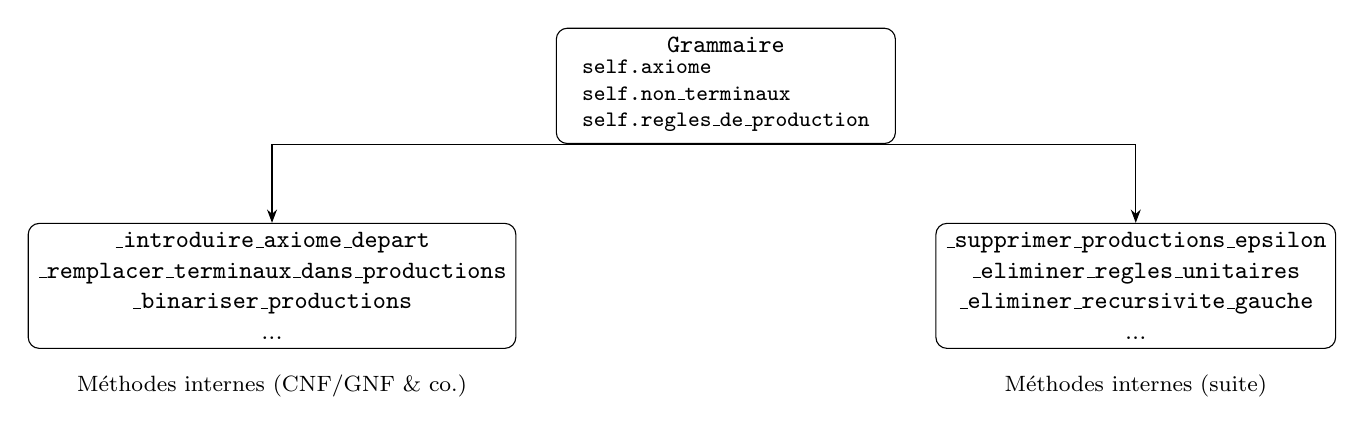
\begin{tikzpicture}[
  font=\small,
  node distance=1.8cm,
  box/.style={draw, rectangle, rounded corners, align=center, minimum width=3cm, minimum height=1cm},
  arrow/.style={->, >=Stealth}
]

% Noeuds
\node[box] (grammar) {\texttt{Grammaire}\\
  \footnotesize
  \begin{tabular}{l}
    \texttt{self.axiome}\\
    \texttt{self.non\_terminaux}\\
    \texttt{self.regles\_de\_production}\\
  \end{tabular}
};

\node[box, below left=1.0cm and 0.5cm of grammar] (method1) {\texttt{\_introduire\_axiome\_depart}\\
\texttt{\_remplacer\_terminaux\_dans\_productions} \\
\texttt{\_binariser\_productions} \\
...};

\node[box, below right=1.0cm and 0.5cm of grammar] (method2) {\texttt{\_supprimer\_productions\_epsilon}\\
\texttt{\_eliminer\_regles\_unitaires}\\
\texttt{\_eliminer\_recursivite\_gauche} \\
...};

% Flèches
\draw[arrow] (grammar.south) -| (method1.north);
\draw[arrow] (grammar.south) -| (method2.north);

\node[below=0.2cm of method1] () {\footnotesize Méthodes internes (CNF/GNF \& co.)};
\node[below=0.2cm of method2] () {\footnotesize Méthodes internes (suite)};

\end{tikzpicture}
} % Fin du \resizebox
\caption{Structure simplifiée de la classe \texttt{Grammaire}, avec ses principaux attributs et méthodes internes.}
\label{fig:diag-grammaire}
\end{figure}


\subsection{Organisation des règles de production}
\label{subsec:organisation-regles}
Concrètement, chaque entrée de \texttt{self.regles\_de\_production} a pour clé un Non-Terminal 
(\emph{exemple} : \texttt{"S0"}) et pour valeur une liste de listes. Par exemple :
\pagebreak 
\begin{lstlisting}[language=python, caption={Exemple de règles de production}, label={lst:regles-production}]
{
    "S0": [
        [("NON_TERMINAL", "A0")],
        [("TERMINAL", "a"), ("NON_TERMINAL", "B1")]
    ],
    "A0": [
        [("EPSILON", "E")]
    ],
    ...
}
\end{lstlisting}

Ici, \texttt{S0} se dérive soit en \texttt{A0}, soit en \texttt{aB1}. Quant à \texttt{A0}, il peut produire la chaîne vide (\texttt{EPSILON}).

\section{Analyseur lexical}
\label{sec:analyseur-lexical}

Pour \textbf{interpréter} les lignes de texte représentant des règles de grammaire (dans un fichier 
\texttt{.general}), nous avons besoin de distinguer différents types de symboles : Non-Terminaux, 
Terminaux, séparateurs de règles, symboles \texttt{EPSILON}, etc. C’est la tâche de l’analyseur lexical 
\texttt{AnalyseurLexical}.

\subsection{Classe \texttt{AnalyseurLexical}}
\label{subsec:classe-analyseur-lexical}

Le fichier \texttt{analyseur\_lexicale.py} définit la classe \texttt{AnalyseurLexical} qui utilise le 
module \texttt{ply.lex} (Python Lex-Yacc) pour mettre en place un lexer. Voici ses principales composantes :

\begin{itemize}
    \item \textbf{Liste des tokens} : 

\begin{lstlisting}[language=python, caption={Extrait du code pour la liste des tokens}, label={lst:tokens}]
tokens = ('REGLE', 'NON_TERMINAL', 'TERMINAL', 'PIPE', 'EPSILON')
\end{lstlisting}

    \item \texttt{t\_REGLE = r':'} : permet de détecter le symbole \texttt{":"}, 
    qui sépare le Non-Terminal à gauche des productions.

    \item \texttt{t\_PIPE = r'\textbackslash{}|'} : 
    pour reconnaître le séparateur \texttt{"|"} entre productions.

    \item \texttt{t\_TERMINAL = r'[a-z]'} : 
    ici, on considère que tout symbole en minuscule sera traité comme un Terminal 
    (ex. \texttt{a}, \texttt{b}, \texttt{c}).

    \item \texttt{t\_EPSILON = r'E'} : 
    ce qui permet de reconnaître le symbole \texttt{"E"} comme \texttt{EPSILON}.

    \item \texttt{t\_ignore = ' \textbackslash{}t'} : 
    pour ignorer les espaces et tabulations.

    \item \texttt{def t\_NON\_TERMINAL(self, t):\\
\quad\quad r'[A-DF-Z]\textbackslash{}s*[0-9]'} : 
    cette méthode spéciale détecte un Non-Terminal, par exemple \texttt{A0} ou \texttt{B1}. 
    L’expression rationnelle autorise une lettre majuscule (sauf \texttt{E} pour éviter la confusion 
    avec \texttt{EPSILON}) suivie d’un chiffre. 
    Au moment de la capture, les espaces intermédiaires sont retirés via 
    \texttt{t.value.replace(' ', '')}.
\end{itemize}

\subsection{Fonctionnement}
\label{subsec:fonctionnement-lexer}
Lorsque l’on appelle la méthode \texttt{analyser\_texte(texte: str)}, le lexer va découper la chaîne 
\texttt{texte} en une suite de \textbf{tokens}. Chaque token contient deux informations essentielles : 
\textbf{type} (ex. \texttt{NON\_TERMINAL}) et \textbf{value} (ex. \texttt{"A0"}). 
Si un caractère non reconnu est rencontré, une exception \texttt{ValueError} est levée pour signaler 
l’erreur (fonction \texttt{t\_error}).

\subsection{Exemple d’analyse lexicale}
\label{subsec:exemple-lexical}
Supposons qu’une ligne du fichier contienne :
\begin{verbatim}
S0 : aB1 | A1
\end{verbatim}
Le lexer va identifier les tokens successifs :
\begin{lstlisting}[language=python, caption={Exemple d’analyse lexicale}, label={lst:exemple-lexical}]
NON_TERMINAL("S0")   # Le Non-Terminal S0
REGLE(":")           # Le symbole de separation :
TERMINAL("a")        # Un Terminal 'a'
NON_TERMINAL("B1")   # Le Non-Terminal B1
PIPE("|")            # Le separateur de production
NON_TERMINAL("A1")   # Le Non-Terminal A1
\end{lstlisting}

Ensuite, chaque production sera traitée pour être stockée dans la \texttt{Grammaire}, 
comme une liste de symboles (voir \ref{subsec:organisation-regles}).

\section{Explications détaillées du code et des algorithmes}
\label{sec:explications-code}

Dans cette section, nous étudions plus en profondeur la structure et le fonctionnement des diverses parties du code, depuis la classe \texttt{Grammaire} (section \ref{subsec:classe-grammaire}) jusqu’aux scripts d’exécution.

\subsection{Organisation générale}
\label{subsec:organisation-generale}

Le projet est organisé en plusieurs fichiers :
\begin{itemize}
    \item \textbf{\texttt{analyseur\_lexical.py}} : contient la classe \texttt{AnalyseurLexical}, chargée de découper chaque ligne de la grammaire en tokens (\texttt{NON\_TERMINAL}, \texttt{TERMINAL}, \texttt{EPSILON}, etc.).
    \item \textbf{\texttt{outil\_grammaire.py}} (ou équivalent) : déclare la classe \texttt{Grammaire} et les fonctions associées \texttt{lire} et \texttt{ecrire}, permettant de lire ou d’écrire des grammaires depuis/vers un fichier.
    \item \textbf{\texttt{grammaire.py}} : script principal qui transforme une grammaire (\texttt{CNF}, \texttt{GNF}) et exporte les résultats.
    \item \textbf{\texttt{generer.py}} : script qui génère des mots à partir de la grammaire, jusqu’à une longueur spécifiée.
\end{itemize}

\noindent
Cette séparation rend le code modulaire et facilite l’utilisation en ligne de commande.

\subsection{La classe \texttt{Grammaire}}
\label{subsec:classe-grammaire-detail}

La classe \texttt{Grammaire}, déjà décrite à la section \ref{subsec:classe-grammaire}, propose des méthodes de transformation (\texttt{CNF}/\texttt{GNF}) et un mécanisme de nettoyage. Nous rappelons seulement qu’elle manipule l’Axiome (\texttt{self.axiome}), l’ensemble de Non-Terminaux (\texttt{self.non\_terminaux}) et les règles de production (\texttt{self.regles\_de\_production}). 

\paragraph{Transformations principales.}
Deux méthodes publiques permettent de convertir la grammaire dans différentes formes normales :

\medskip

\textbf{1) \texttt{convertir\_en\_forme\_normale\_de\_Chomsky() (CNF)}}.\\
Cette méthode introduit d’abord un nouvel axiome (étape \emph{START}), puis remplace les terminaux dans les productions de longueur supérieure à 1 (étape \emph{TERM}), avant de binariser les productions (\emph{BIN}). Ensuite, elle supprime les productions \(\epsilon\) si nécessaire (\emph{DEL}) et élimine les règles unitaires (\emph{UNIT}). Au terme de ces étapes, la grammaire respecte la définition de la CNF : les productions sont soit de la forme \(\;A \to BC\), soit \(\;A \to a\), soit \(\;S \to \epsilon\) si l’axiome est nullable.

\bigskip

\textbf{2) \texttt{convertir\_en\_forme\_normale\_de\_Greibach() (GNF)}}.\\
Pour atteindre la GNF, la méthode introduit d'abord un nouvel axiome (similaire à \emph{START} en CNF). Ensuite, elle supprime les \(\epsilon\)-productions (étape \emph{DEL}) et enlève les règles unitaires (\emph{UNIT}). Puis elle élimine toute récursivité gauche (directe ou indirecte). Enfin, elle assure que chaque production commence par un terminal : la procédure  \texttt{\_supprimer\allowbreak\_non\allowbreak\_terminaux\allowbreak\_en\allowbreak\_tete\allowbreak\_des\allowbreak\_regles()} \emph{“déplie”} tout non-terminal placé au début d’une règle, et la procédure \texttt{\_supprimer\_symboles\_terminaux\_non\_en\_tete()} remplace tout terminal placé après le premier symbole par un nouveau non-terminal dédié (ex. \texttt{T\_b -> b}). Ainsi, toutes les règles prennent la forme \(\,A \to a\,A_1\,\dots\,A_k\) (ou \(\epsilon\) si l’axiome peut être vide).

\paragraph{Méthodes internes (privées) :}
\begin{itemize}
    \item \texttt{\_introduire\_axiome\_depart()} : crée un nouveau Non-Terminal pour pointer vers l’ancien Axiome.
    \item \texttt{\_remplacer\_terminaux\_dans\_productions(...)} : déplace les \texttt{TERMINAL} vers des règles dédiées (ex. \texttt{T\_a -> a}) pour la \texttt{CNF} ou la \texttt{GNF}.
    \item \texttt{\_binariser\_productions()} : découpe toute production de plus de deux symboles en productions binaires (ex. \texttt{S -> A X}, \texttt{X -> B C}).
    \item \texttt{\_supprimer\_productions\_epsilon()} : identifie les Non-Terminaux \emph{annulables} (\texttt{EPSILON}) et supprime les règles vides, sauf si l’Axiome est concerné.
    \item \texttt{\_eliminer\_regles\_unitaires()} : remplace \texttt{X -> Y} (un seul Non-Terminal) par les productions de \texttt{Y}.
    \item \texttt{\_eliminer\_recursivite\_gauche()} : gère la récursivité gauche directe (\texttt{A -> A ...}) et indirecte (\texttt{A -> B, B -> A}).
    \item \texttt{\_supprimer\_non\_terminaux\_en\_tete\_des\_regles()} : pour chaque production \texttt{X -> Y} $\alpha$ (avec \texttt{Y} un \texttt{NON\_TERMINAL}), remplace \texttt{X -> Y} $\alpha$ par \texttt{X -> (p)} $\alpha$ pour chacune des productions \texttt{p} de \texttt{Y},  jusqu’à ce qu’aucune règle ne commence plus par un \texttt{NON\_TERMINAL}.
    \item \texttt{\_supprimer\_symboles\_terminaux\_non\_en\_tete()} : transforme tout \texttt{TERMINAL} (au-delà du premier symbole) en un nouveau \texttt{NON\_TERMINAL} dédié (ex. \texttt{T\_b -> b}). Ainsi, chaque production commence par un \texttt{TERMINAL}, et les symboles suivants sont uniquement des \texttt{NON\_TERMINAL}.
\end{itemize}


\paragraph{Nettoyage (\texttt{nettoyer\_grammaire()}) :}
La classe \texttt{Grammaire} inclut aussi des fonctions pour supprimer les Non-Terminaux inaccessibles, vides ou non-productifs :  
\begin{itemize}
    \item \texttt{supprimer\_non\_terminaux\_vides()},
    \item \texttt{supprimer\_non\_productifs()},
    \item \texttt{supprimer\_non\_terminaux\_inaccessibles()}.
\end{itemize}

\subsection{Génération dynamique de nouveaux Non-Terminaux}
Pour les transformations \texttt{CNF} ou \texttt{GNF}, il peut être nécessaire de créer des symboles Non-Terminaux \emph{temporaires}. La fonction \texttt{generer\_non\_terminal(non\_terminaux)} génère un nom du type \texttt{"A0"}, \texttt{"B0"}, etc., en évitant les collisions avec l’ensemble existant.

\subsection{Détails sur les transformations CNF et GNF}
\label{subsec:details-cnf-gnf}

Au-delà du simple appel aux méthodes \texttt{convertir\_en\_forme\_normale\_de\_Chomsky()} et \texttt{convertir\_en\_forme\_normale\_de\_Greibach()}, nous détaillons ici les différentes étapes suivies pour chaque forme normale.

\subsubsection{Forme Normale de Chomsky (CNF)}

Une grammaire est dite en \emph{Forme Normale de Chomsky} si toutes ses productions vérifient l’un des trois types :
\begin{enumerate}
    \item \(A \to BC\), où \(A, B, C\) sont des non-terminaux (pas d’autres symboles),
    \item \(A \to a\), où \(a\) est un terminal,
    \item (Optionnel) \(S \to \epsilon\) (production vide) seulement si l’axiome \(S\) est nullable.
\end{enumerate}

Notre méthode \texttt{convertir\_en\_forme\_normale\_de\_Chomsky()} applique successivement :
\begin{enumerate}
    \item \textbf{START} : on introduit un nouvel axiome \(\texttt{S'}\) pour éviter les cas où l’axiome initial est présent à droite de certaines règles. Concrètement, si l’axiome initial est \(S0\), on crée \(S' \to S0\).  
    \item \textbf{TERM} : on remplace les terminaux dans les productions de longueur \(> 1\) par des non-terminaux dédiés. Par exemple, si une production contient \(\ldots a \ldots\), on crée un nouveau non-terminal \(\texttt{A\_a}\) tel que \(\texttt{A\_a} \to a\), et on remplace \(a\) par \texttt{A\_a}.  
    \item \textbf{BIN} : on binarise toutes les productions qui ont plus de deux symboles. Par exemple, \(S \to A B C\) devient \(S \to A X\) et \(X \to B C\). Le code parcourt récursivement les productions afin de créer de nouveaux non-terminaux si nécessaire.  
    \item \textbf{DEL} : on supprime les \(\epsilon\)-productions (c’est-à-dire les règles produisant la chaîne vide). On identifie d’abord tous les non-terminaux \emph{nullables}, puis on génère toutes les variantes des productions sans ces non-terminaux, sauf si l’axiome lui-même est nullable (dans ce cas, on autorise \(\epsilon\) uniquement pour l’axiome).  
    \item \textbf{UNIT} : on élimine les règles unitaires (de la forme \(A \to B\)). Pour cela, on remplace \(A \to B\) par l’ensemble des productions de \(B\).  
\end{enumerate}

Une fois ces étapes réalisées dans l’ordre indiqué, la grammaire obtenue est en CNF : toute production aura soit deux non-terminaux (type \(A \to BC\)), soit un terminal isolé (type \(A \to a\)), soit éventuellement \(\epsilon\) si l’axiome est nullable.

\subsubsection{Forme Normale de Greibach (GNF)}

Une grammaire est dite en \emph{Forme Normale de Greibach} si toutes ses productions commencent par un \textbf{terminal}, éventuellement suivi d’une suite (éventuellement vide) de non-terminaux. Formellement, toute règle est du type :
\[
A \to a \, X_1 X_2 \ldots X_k
\]
où \(a\) est un terminal, et chaque \(X_i\) est un non-terminal. En plus, on autorise \(S \to \epsilon\) si l’axiome \(S\) peut produire la chaîne vide.

Notre méthode \texttt{convertir\_en\_forme\_normale\_de\_Greibach()} procède ainsi :
\begin{enumerate}
    \item \textbf{START} : introduction d’un nouvel axiome \texttt{S'}.
    \item \textbf{DEL} : suppression des \(\epsilon\)-productions (sauf si l’axiome est nullable).
    \item \textbf{UNIT} : élimination des règles unitaires X→YX→Y.
    \item \textbf{Élimination de la récursivité gauche} (directe et indirecte).
    \item\textbf{SUPPRIMER\_NON\_TERMINAUX\_EN\_TÊTE} : forcer chaque règle à débuter par un terminal.
    \item \textbf{SUPPRIMER\_TERMINAUX\_NON\_EN\_TÊTE} : remplacer tout terminal situé après le premier symbole par un non-terminal dédié.
\end{enumerate}

Ainsi, chaque règle débute par un unique terminal. Toute éventuelle récursivité gauche a été éliminée.

\subsection{Lecture et écriture de la grammaire : \texttt{lire} et \texttt{ecrire}}
\label{subsec:lire-ecrire}

\paragraph{\texttt{lire(fichier: str) -> Grammaire}} 
\begin{enumerate}
    \item Crée un \texttt{AnalyseurLexical()} pour analyser chaque ligne en tokens.
    \item Instancie une \texttt{Grammaire}.
    \item Parcourt le fichier \texttt{.general}, construit les productions et détecte le Non-Terminal de gauche.
    \item Nettoie la grammaire via \texttt{nettoyer\_grammaire()} et renvoie l’objet \texttt{Grammaire}.
\end{enumerate}

\paragraph{\texttt{ecrire(grammar, fichier\_base, extension)}} 
\begin{enumerate}
    \item Construit un fichier de sortie (\texttt{.chomsky} ou \texttt{.greibach}).
    \item Écrit d’abord l’Axiome et ses productions, puis les autres Non-Terminaux triés.
    \item Pour chaque production, on concatène les symboles (ex. \texttt{X1}, \texttt{a}, \texttt{E}) en séparant par \texttt{|} si nécessaire.
\end{enumerate}

\subsection{Script \texttt{grammaire.py} : transformations}
\label{subsec:grammaire-py}

Ce script :
\begin{enumerate}
    \item Lit le fichier \texttt{.general} donné en argument.
    \item Copie la \texttt{Grammaire} pour appliquer deux transformations : \texttt{convertir\_en\_forme\_normale\_de\_Chomsky()} et \texttt{convertir\_en\_forme\_normale\_de\_Greibach()}.
    \item Écrit les grammaires transformées dans \texttt{.chomsky} et \texttt{.greibach}.
\end{enumerate}

\subsection{Script \texttt{generer.py} : génération de mots}
\label{subsec:generer-py}

Le script \texttt{generer.py} sert à tester la grammaire en générant les mots reconnus jusqu’à une longueur donnée.

\paragraph{\texttt{generer\_mots(longueur: int)}} 
\begin{itemize}
    \item Démarre depuis l’Axiome, explore toutes les productions (méthode récursive).
    \item Ajoute les \texttt{TERMINAL}, déplie les \texttt{NON\_TERMINAL} et ignore \texttt{EPSILON}.
    \item Stocke chaque mot final (entièrement dérivé) dans un \texttt{set} pour éviter les doublons.
    \item Renvoie la liste triée (ou signale qu’aucun mot n’est généré).
\end{itemize}

\noindent
Exemple de commande :
\begin{lstlisting}[language=bash, caption={Exemple d’utilisation de generer.py}, label={lst:exemple-generer}]
$ python generer.py 3 exemple.general
\end{lstlisting}
Cette commande affiche tous les mots de longueur \(\leq 3\) produits par la grammaire contenue dans \texttt{exemple.general}.

\subsection{Fichiers de test (\texttt{test.general})}
\label{subsec:tests}

En plus des fichiers requis ( \texttt{3.general}, \texttt{4.general} et \texttt{5.general}), deux fichiers de test ont été préparés, nommés \texttt{1.general} et \texttt{2.general}, et correspondant à différentes grammaires.

\begin{table}[h!]
\centering
\renewcommand{\arraystretch}{1.2}
\begin{tabular}{|c|l|p{7cm}|}
\hline
\texttt{1.general} & \begin{minipage}[t]{0.27\textwidth}
\texttt{S0 : A1S0B1 | C1\\
A1 : a\\
B1 : b\\
C1 : c | E}
\end{minipage}
& Mots de la forme \(a^n c b^n\) ou un simple \texttt{c}. \\
\hline
\texttt{2.general} & \begin{minipage}[t]{0.27\textwidth}
\texttt{S0 : A1S0A1 | B1S0B1 | E | A1 | B1\\
A1 : a\\
B1 : b}
\end{minipage}
& Palindromes en \texttt{a} et \texttt{b}. \\
\hline
\end{tabular}
\caption{Récapitulatif des fichiers de test \texttt{.general} et des langages correspondants.}
\label{tab:recap-general}
\end{table}

Ces différents fichiers permettent de tester le \textbf{pipeline complet} (lecture, transformation, génération de mots) sur des grammaires variées, incluant des langages vides, des combinaisons de lettres, ou des palindromes.

\subsection{Conclusion}
\label{subsec:conclusion}

Avec ces scripts, on dispose d’un \textbf{pipeline complet} pour :
\begin{enumerate}
    \item Lire une grammaire (\texttt{.general}).
    \item \textbf{Analyser} lexicalement et la convertir en une structure \texttt{Grammaire}.
    \item Appliquer des \textbf{transformations} en formes normales (\texttt{CNF}, \texttt{GNF}).
    \item \textbf{Générer} des mots pour valider la grammaire.
\end{enumerate}

L’ensemble permet d’explorer, de tester et de manipuler différentes grammaires contextuelles de manière modulaire et extensible.

% --- DIAGRAMME DU PIPELINE ---

\begin{figure}[h!]
\centering
\resizebox{0.92\textwidth}{!}{%
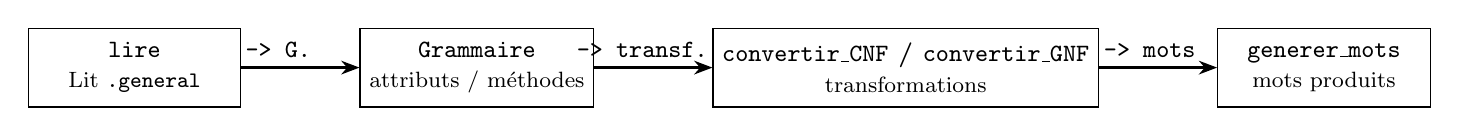
\begin{tikzpicture}[
  font=\small,
  node distance=1.5cm,
  stepnode/.style={
    draw, 
    rectangle, 
    align=center, 
    minimum width=2.7cm, 
    minimum height=1cm
  },
  arrow/.style={->, >=Stealth, thick}
]

% Noeuds
\node[stepnode] (read) {\textbf{\texttt{lire}}\\
\footnotesize Lit \texttt{.general}};
\node[stepnode, right=of read] (grammar) {\textbf{\texttt{Grammaire}}\\
\footnotesize attributs / méthodes};
\node[stepnode, right=of grammar] (transform) {\textbf{\texttt{convertir\_CNF} / \texttt{convertir\_GNF}}\\
\footnotesize transformations};
\node[stepnode, right=of transform] (generate) {\textbf{\texttt{generer\_mots}}\\
\footnotesize mots produits};

% Flèches
\draw[arrow] (read) -- (grammar) 
  node[midway, above, xshift=-0.8em]{\texttt{-> G.}};
\draw[arrow] (grammar) -- (transform) 
  node[midway, above, xshift=-0.4em]{\texttt{-> transf.}};
\draw[arrow] (transform) -- (generate) 
  node[midway, above, xshift=-0.3em]{\texttt{-> mots}};

\end{tikzpicture}
}% % Fin du \resizebox
\caption{Pipeline général : lecture (\texttt{lire}) \(\to\) création d’une \texttt{Grammaire} \(\to\) transformations CNF/GNF \(\to\) génération de mots.}
\label{fig:pipeline}
\end{figure}

\section{Gestion du projet et automatisation}
\label{sec:makefile-req}

\subsection{Le \texttt{Makefile}}
\label{subsec:makefile}

Pour faciliter la génération et les tests autour de la grammaire, un fichier \texttt{Makefile} est fourni. Il définit plusieurs cibles (\texttt{all}, \texttt{test}, \texttt{clean}, \ldots) et automatise l’exécution des scripts \texttt{grammaire.py} (section \ref{subsec:grammaire-py}) et \texttt{generer.py} (section \ref{subsec:generer-py}). Voici ses principales fonctionnalités :

\begin{itemize}
    \item \textbf{\texttt{make}} : Génère automatiquement les fichiers \texttt{.chomsky} et \texttt{.greibach} à partir de tous les fichiers \texttt{.general} détectés dans le répertoire. Concrètement, il invoque :
\begin{lstlisting}[language=bash, caption={Extrait de Makefile pour la cible `all`}, label={lst:make-all}]
python grammaire.py <fichier.general>
\end{lstlisting}

    \item \textbf{\texttt{make N=<longueur> test}} : Teste la génération de mots à partir de chaque fichier \texttt{.chomsky} et \texttt{.greibach}, pour une longueur de mots \textbf{obligatoirement spécifiée} par \texttt{N=<longueur>}.  
    Par exemple, \texttt{make N=5 test} indiquera de générer des mots de longueur 5. Il appelle en interne :
\begin{lstlisting}[language=bash, caption={Extrait de Makefile pour la cible `test`}, label={lst:make-test}]
python generer.py <longueur> <fichier.chomsky> > base_<longueur>_chomsky.res
python generer.py <longueur> <fichier.greibach> > base_<longueur>_greibach.res
diff -u base_<longueur>_chomsky.res base_<longueur>_greibach.res
\end{lstlisting}

    afin de comparer les résultats \texttt{\_chomsky.res} et \texttt{\_greibach.res}.

    \item \textbf{\texttt{make clean}} : Supprime tous les fichiers générés (\texttt{.chomsky}, \texttt{.greibach}, \texttt{\_chomsky.res}, \texttt{\_greibach.res}).

    \item \textbf{\texttt{make help}} : Affiche un résumé des différentes commandes proposées et rappelle qu’il faut spécifier \texttt{N=<longueur>} pour \texttt{test} et \texttt{clean}.
\end{itemize}

\subsection{Les dépendances : \texttt{requirements.txt}}
\label{subsec:requirements}

Le fichier \texttt{requirements.txt} répertorie les bibliothèques Python nécessaires au bon fonctionnement du projet. Dans notre cas, il se limite principalement à :

\begin{lstlisting}[language=bash, caption={requirements.txt}, label={lst:requirements}]
ply~=3.11
\end{lstlisting}

Cela indique que nous utilisons la bibliothèque \texttt{ply} (version 3.11 ou approchante). Pour installer automatiquement cette dépendance, vous pouvez utiliser la commande :
\begin{lstlisting}[language=bash, caption={Installation des dépendances}, label={lst:install}]
pip install -r requirements.txt
\end{lstlisting}

\paragraph{Version de Python}
Ce projet a été développé et testé avec \textbf{Python 3.11}.

\end{document}
